% Thanks to http://tex.stackexchange.com/a/30782/5645 for this
% example!
\documentclass{article}
\usepackage{amsmath}
\usepackage{ amssymb}
\usepackage{mathptmx}
\usepackage{tikz}
\usepackage{pgfplots}
%\usepgfplotslibrary{polar}
\usepackage{tkz-fct}
\usetikzlibrary{angles, quotes}
\usetikzlibrary{arrows.meta, arrows}
\usetikzlibrary{shapes.geometric}
\usetikzlibrary{external}
\tikzexternalize[prefix={external/}]

\tikzset{
    export as png/.style={
        external/system call/.add={}{
            && convert -density #1 -transparent white "\image.pdf" "\image.png"
        },
    },
    export as png/.default={200},
    % Arrow tips
    >=stealth,
}

% pgfplots settings
\input{colors}
\input{pgfplots}

\DeclareSymbolFont{symbolsb}{OMS}{cmsy}{m}{n}
\SetSymbolFont{symbolsb}{bold}{OMS}{cmsy}{b}{n}
\DeclareSymbolFontAlphabet{\mathcal}{symbolsb}

\def\req{\protect\rotatebox{90}{$\scriptstyle=$}}

\newcommand{\addaxes}{\draw (0em,1em) -- (0em,-1em)
                            (-1em,0em) -- (1em,0em);}
\newcommand{\stepfunc}{\draw[line width=1.5pt] (0.65em,0.65em) -- (0,0.65em) 
                                    -- (0,-0.65em) -- (-0.65em,-0.65em);}

\begin{document}

\tikzset{export as png}

\tikzsetnextfilename{perceptron}
% Author: Alfredo Sánchez Alberca (asalber@ceu.es)
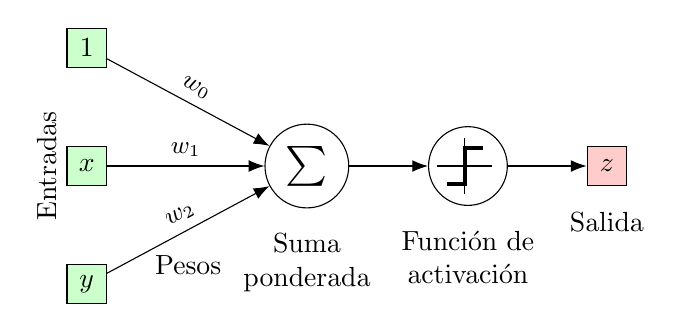
\begin{tikzpicture}[
    node distance=1.5cm,
    neuron/.style={circle, draw, minimum size=1cm},
    input/.style={rectangle, draw, minimum size=0.5cm, fill=green!20},
    output/.style={rectangle, draw, minimum size=0.5cm, fill=red!20},
    weight/.style={font=\small, midway, above, sloped}
]

% Input neurons
\node[input] (in1) {1};
\node[input, below of=in1] (in2) {$x$};
\node[input, below of=in2] (in3) {$y$};

% Output neuron
\node[neuron, right=2cm of in2] (out) {\Large $\sum$};

% Connect inputs to output
\draw[-{Latex[length=2mm]}] (in1) -- (out) node[weight] {$w_0$};
\draw[-{Latex[length=2mm]}] (in2) -- (out) node[weight] {$w_1$};
\draw[-{Latex[length=2mm]}] (in3) -- (out) node[weight] (w2) {$w_2$};

% Activation function
\node[neuron, right=1cm of out] (activation) {};
\draw[-{Latex[length=2mm]}] (out) -- (activation);
\begin{scope}[xshift=4.8cm, yshift=-1.5cm, scale=1]
    \addaxes;
    % flexible selection of activation function
    % \relu
    \stepfunc;
\end{scope};

% Output function 
\node[output, right=1cm of activation] (output) {$z$};
\draw[-{Latex[length=2mm]}] (activation) -- (output);

% Etiquetas
\node[left=5mm of in2, rotate=90, anchor=north] {Entradas};
\node[below=2mm of output] {Salida};
\node[below=2mm of w2] {Pesos};
\node[below=2mm of out, align=center] {Suma\\ponderada};
\node[below=2mm of activation, align=center] {Función de\\activación};
\end{tikzpicture}
   

\end{document}